%!TEX root = ../thesis.tex
%*******************************************************************************
%****************************** Sixth Chapter **********************************
%*******************************************************************************
\chapter{Implementation}

\graphicspath{{Chapter6/Figs/Raster/}{Chapter6/Figs/}}

\section{Development Environment and Tools}

\begin{figure}[!ht] 
    \centering    
    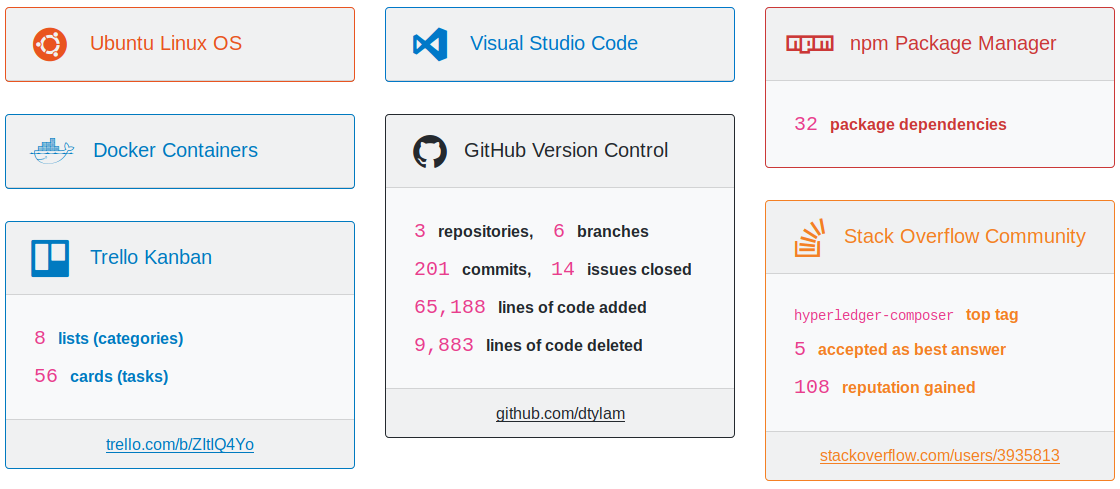
\includegraphics[width=1.0\textwidth]{platform_stats}
    \caption[Development Tools and Usage Statistics]
        {A visual overview of the tools used and their usage statistics if any} 
    \label{fig:platform_stats}
\end{figure}

Specific systems and tools were used to build the demonstrator network and client applications (as in Figure \ref{fig:platform_stats}). 
These choices and their rationale are detailed below:

\underline{Operating System}: The developer's guide for both Hyperledger Composer and Hyperledger Fabric 
recommends using Ubuntu or Mac OS as the host operating system for development. 
Ubuntu is selected for being the free and open source option. The development personal computer, which was originally 
a Windows machine, was set up to dual boot with the latest Ubuntu release.

\underline{Version Control}: A version control system or software keeps track of source code modifications, 
so that developers can compare earlier versions of the code, revert changes, and 
minimise disruptions of mistakes \citep{atlassian2018vcs}. It is essential to medium to large scaled projects.

All work done at the implementation stage was tracked with the version control system Git. 
Git is a distributed version control system, where repositories can be backed up to a remote server, 
such as on the cloud. This is done with GitHub, a git-based version control, code hosting and 
project management service that offers free private repositories to verified students \citep{github2018education}.

\underline{Code Editor}: The Hyperledger Composer framework does not require a dedicated integrated 
development environment and recommends using a text editor. Visual Studio Code, an open source text editor developed 
by Microsoft was chosen as it has a dedicated syntax checking and beautifying official plugin for Hyperledger Composer.

\underline{Community Support}: Hyperledger Composer and Hyperledger Fabric have active communities on Stack Overflow, 
a popular online community forums for developers to discuss coding problems. Throughout the duration of the project, 
it has been a source of solutions to common problems faced and solved by many other users. Towards the end of the project, 
answer contributions were also made.

Several other tools were also used, for example, as previously mentioned in Chapter 3, Trello was used to manage 
feature prioritisation for the agile development process. The use of Docker containers and npm package manager 
will be explained in due course below.

\section{Architecture and Tech Stack}

\begin{figure}[!ht] 
    \centering    
    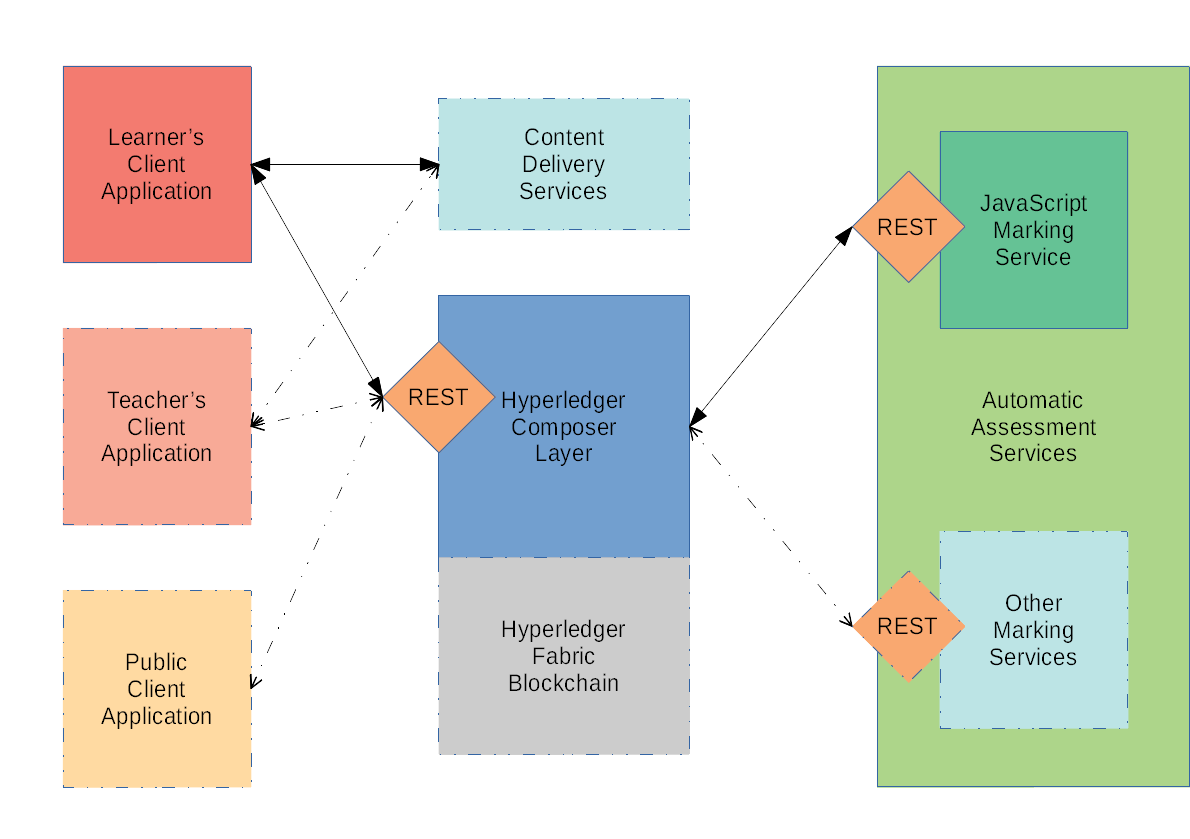
\includegraphics[width=1.0\textwidth]{architecture}
    \caption[Component architecture overview for the demonstrator system built]
        {Component architecture overview for the demonstrator system built}
    \label{fig:architecture}
\end{figure} 

\begin{figure}[!ht] 
    \centering    
    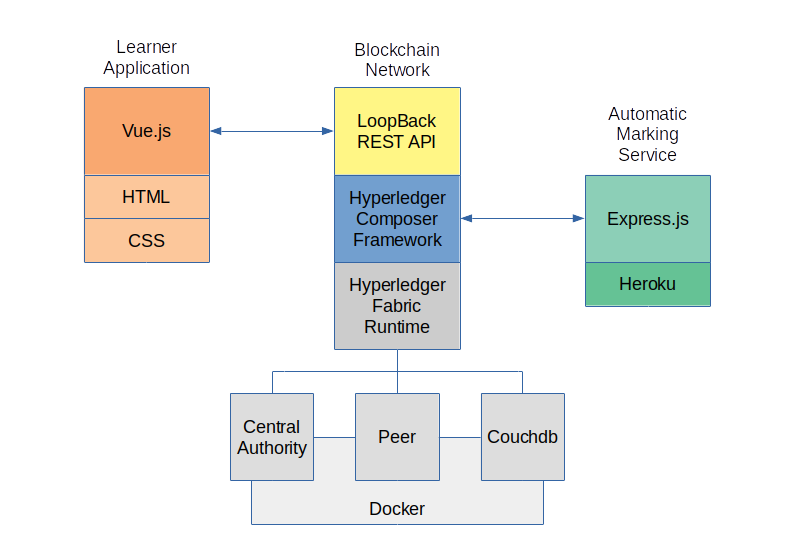
\includegraphics[width=0.9\textwidth]{techstack}
    \caption[Technology Stack overview for the demonstrator system built]
        {Technology Stack overview for the demonstrator system built}
    \label{fig:techstack}
\end{figure} 

\section{Docker and the Command Line Interface}

\section{Application Program Interface}

\section{Learner Client Application}

\section{Teacher Client Application}

